% This must be in the first 5 lines to tell arXiv to use pdfLaTeX, which is strongly recommended.
%\pdfoutput=1
% In particular, the hyperref package requires pdfLaTeX in order to break URLs across lines.

\documentclass[11pt]{article}

% Remove the "review" option to generate the final version.
\usepackage[review]{acl}

% Standard package includes
\usepackage{times}
\usepackage{latexsym}
\usepackage{newunicodechar}

% For proper rendering and hyphenation of words containing Latin characters (including in bib files)
\usepackage[T1]{fontenc}
% For Vietnamese characters
% \usepackage[T5]{fontenc}
% See https://www.latex-project.org/help/documentation/encguide.pdf for other character sets

% This assumes your files are encoded as UTF8
\usepackage[utf8]{inputenc}

% This is not strictly necessary, and may be commented out,
% but it will improve the layout of the manuscript,
% and will typically save some space.
\usepackage{microtype}

\usepackage{amsmath}
\usepackage{amssymb}
\usepackage{siunitx}
\usepackage{booktabs}
\usepackage{pgfplots}
\usepackage{todonotes}
\usepackage{enumitem}
\usepackage{cleveref}
\usepackage{array}
\usepackage{makecell}
\usepackage{multirow}

\usepgfplotslibrary{groupplots}
\usepgfplotslibrary{statistics}
\pgfplotsset{compat=1.16}
\pgfplotsset{every tick label/.append style={font=\footnotesize}}

\renewcommand{\UrlFont}{\ttfamily\small}

\newcommand\jp[1]{\todo[backgroundcolor=blue!10]{JP: #1}}
\newcommand\bn[1]{\todo[backgroundcolor=green!10]{BN: #1}}



\newcommand\Ppl{\mathsf{Ppl}}
\newcommand\IG{\mathsf{IG}}
\newcommand\Ind{\mathsf{Ind}}
\newcommand\LM{\mathrm{LM}}
\newcommand\CCLM{\mathrm{CCLM}}
\DeclareMathOperator*{\avg}{average}
\newcommand\BibTeX{B\textsc{ib}\TeX}
\newcommand\subreddit[1]{\texttt{/r/#1}}
\newlist{hypotheses}{enumerate}{3}
\setlist[hypotheses,1]{parsep=0pt,itemsep=1pt,font=\bfseries,label=(H\arabic*)}

\newcommand{\commpcaplot}[1]{%
  \addplot[
  scatter, only marks,
  font=\tiny,
  scatter src=explicit symbolic,
  scatter/classes={
    general-interest={mark=*, blue},
    videogames={mark=*, red},
    technology={mark=*, green},
    sports={mark=*, cyan},
    female-focused={mark=*, magenta},
    other={mark=o, black}%
  },
  nodes near coords*={\community},
  visualization depends on={value \thisrow{community} \as \community}
  ] table [x=pca1, y=pca2, meta=category] {#1};
}

\newcommand{\commpcagroupplot}[2]{%
  \begin{groupplot}[
    group style={group size=2 by 1}, 
    yticklabels={,,}, xticklabels={,,},
    legend style={anchor=north, legend columns=1, font=\tiny},
    every node near coord/.append style={font=\sffamily\tiny}%
    ]
    \nextgroupplot
    \commpcaplot{#1}
    \nextgroupplot
    \commpcaplot{#2}
    \legend{General interest,Videogames,Technology,Sports,Female-focused,Other}
  \end{groupplot}
}

\newcommand{\confusionplot}[1]{%
  \addplot[
  matrix plot*,
  shader=faceted,
  mesh/cols=46,
  point meta=explicit,
  ] table [x=actual_comm, y=pred_comm, meta=#1] {floats/confusion.csv};
}

\newcommand{\confusiongroupplot}[2]{%
  \begin{groupplot}[
    group style={group size=2 by 1}, 
    enlargelimits=false,
    axis line style={draw=none},
    %axis equal,
    xmin=-1, xmax=46,
    ymin=-1, ymax=46,
    width=8cm,
    xticklabels={Advice,AskWomen,BabyBumps,CFB,Drugs,EDH,EarthPorn,Fantasy,GameDeals,GlobalOffensive,Jokes,Kappa,KerbalSpaceProgram,KotakuInAction,LifeProTips,MLS,MMA,MaddenUltimateTeam,TwoXChromosomes,Warframe,airsoft,bodybuilding,breakingmom,cars,cringe,eu4,exjw,explainlikeimfive,femalefashionadvice,food,heroesofthestorm,jailbreak,justneckbeardthings,oculus,pcmasterrace,photography,reddevils,relationships,rupaulsdragrace,stopdrinking,streetwear,techsupport,todayilearned,toronto,videos,xxfitness},
    yticklabels=none,
    xticklabel style={font=\sffamily\tiny, rotate=90},
    xtick=data,
    legend style={font=\sffamily\small},
    ]
    \nextgroupplot
    \confusionplot{#1}
    \nextgroupplot[colorbar right]
    \confusionplot{#2}
  \end{groupplot}
}

\newcommand{\pairwisecommsim}[1]{%
  \begin{tikzpicture}
    \begin{axis}[]
      \addplot[
        scatter, only marks,
        font=\tiny,
        scatter src=explicit symbolic,
        scatter/classes={
          general-interest={mark=*, blue},
          videogames={mark=*, red},
          technology={mark=*, green},
          sports={mark=*, cyan},
          female-focused={mark=*, magenta},
          other={mark=o, black},
          different={mark=x}
        },
        ] table [x=snap, y=#1, meta=meta] {floats/comm_sim.csv};
    \end{axis}
  \end{tikzpicture}
}

\newcommand{\pplscatter}[2]{%
  \begin{tikzpicture}
  \begin{axis}[]
  \addplot[
    only marks, black,
  ] table [x=#1, y=#2] {floats/cclm_lmcc_ppl.csv};
  \end{axis}
  \end{tikzpicture}
}





\title{Community-Conditioned Language Models}

% Author information can be set in various styles:
% For several authors from the same institution:
% \author{Author 1 \and ... \and Author n \\
%         Address line \\ ... \\ Address line}
% if the names do not fit well on one line use
%         Author 1 \\ {\bf Author 2} \\ ... \\ {\bf Author n} \\
% For authors from different institutions:
% \author{Author 1 \\ Address line \\  ... \\ Address line
%         \And  ... \And
%         Author n \\ Address line \\ ... \\ Address line}
% To start a seperate ``row'' of authors use \AND, as in
% \author{Author 1 \\ Address line \\  ... \\ Address line
%         \AND
%         Author 2 \\ Address line \\ ... \\ Address line \And
%         Author 3 \\ Address line \\ ... \\ Address line}

\author{First Author \\
  Affiliation / Address line 1 \\
  Affiliation / Address line 2 \\
  Affiliation / Address line 3 \\
  \texttt{email@domain} \\\And
  Second Author \\
  Affiliation / Address line 1 \\
  Affiliation / Address line 2 \\
  Affiliation / Address line 3 \\
  \texttt{email@domain} \\}

\date{}

\begin{document}
\maketitle
\begin{abstract}

  TODO: fix this up.
  % Context (Optional)

  % Problem?

  - Can community-level linguistic variation be captured by statistical models?
  
  - Is community-specific linguistic variation correlated with social
    relationship between communities?
  
  % Why it's interesting


  % Results


  % What follows from results? (Optional)
    
  Community-Conditioned Language Models (CCLMs) are an under-researched tool for 
  investigating community-level linguistic variation.
  In this paper, we experiment with different neural CCLM architectures and
  report empirical results from CCLMs trained on 510 online communities.
  We find that the community embeddings learned by these models
  correlate with representations based on non-linguistic features.
  We define a metric of the linguistic \emph{indiscernability} of a community
  and investigate the relationship between indiscernibility and other
  linguistic properties of the community.
\end{abstract}


% Introduction

% Community Conditioned Language Models:
%   Data sets
%   Architecture (with emphasis on the embeddings)
%   Training
%   Results (loss and loss per community)

% Latent bayesian community classifier
%    Formula (no training!)
%    Result 1: Confusion matrix
%    Transition: too much data; can we extract a more useful metric?
%    Indiscernibility: Formula, and table

% Correlation between linguistic embedding with social embeddings
%    Kumar2018 Data set
%    Explain the problem (idea: comparing cosine similarities --> too much data, again)
%    Sketch "procrustes" problem, explain what it yields. (Also what kind of similarity one gets with random input)
%    Results:
%      - Correlation between Kumar2018 and best LSTM
%      - Correlation between Kumar2018 and best Transformer 
%      - Correlation between Transformer and LSTM
%      - Concatenations ???



\section{Introduction}
Linguistic communication requires that speakers share
knowledge of certain linguistic conventions, such as syntactic
structure, word meanings, and accepted patterns of interaction.
Speakers assume that these conventions are \emph{common ground} among
their interlocutors, based on joint membership in a community
\cite{Stalnaker2002, Clark1996}.  Such a community may be of any size,
from the very small, like members of a particular friend group, to the
very large, like speakers of English.  Because it is the source of
linguistic convention, the \emph{speech community} is an important
concept in the study of linguistic variation \citep{Gumperz1972}.

% Not only is linguistic variation an object of inquiry in its own
% right, but it is also important to consider it in the development of
% robust, equitable language technology.  Previous work has shown that
% by taking demographic information into account, models can achieve
% better performance on various standard NLP tasks
% \citep{Hovy2015,Yang2017}. \jp{Move this to related work so we can get to the point quicker.}
=
Most of the previous computational work on linguistic variation 
has considered variation at the level of macro-social categories, such as gender
\citep{Burger2011,Ciot2013,Bamman2014}, age \citep{Nguyen2013}, and
geographic location \citep{Eisenstein2010,Bamman2014a}.
An exception is \citet{DelTredici2017} who use the modified
skip-gram model of \citet{Bamman2014a} to show that lexical semantic
variation occurs across different communities organized around the
same topic.

In the present work, we investigate linguistic variation
across different online communities. In contrast to previous work, we
investigate variation across speech communities (rather than
macro-social categories), and use context-sensitive sequence models
capable of capturing variation beyond the lexical level.
%
We do so by investigating two questions.  First, we are interested in
variation in the level of \emph{linguistic complexity}
exhibited by different communities.\footnote{
  We will define linguistic complexity as language model perplexity.
  We do not intend to make any claim about the relationhip
  between language model perplexity and other notions of linguistic
  complexity \citep[cf.][]{Hawkins2014}. Furthermore, we note that 
  language \emph{exhibited} by a speech community \citep[i.e., \emph{parole},][]{deSaussure2011}
  is  different from \emph{a language} (i.e., \emph{langue}).}
%\jp{
  %Some examples (perhaps include if there is space):
  
  %(CFB)
  %It was against SMU in the 47-48 Cotton bowl. They had cancelled a
  %game the year before against Miami for the same reason. There's
  %debate on if that's really the origin for the phrase but the story
  %itself is true.

  %(Videos)
  %Reminds me of Y2K computer bug. A lot of work went into
  %pre-emptively fixing it, and a lot of bugs were found and fixed,
  %some of which would have been catastrophic. Unfortunately, because
  %the work was successful, a lot of people now describe it as a waste
  %of time/money and a big deal made out of nothing.  }
%
Indeed, it is folklore that certain communities tend to exhibit more predictable
speech patterns than others.  Here we want to quantify this
phenomenon.  More precisely, we investigate if the degree of
complexity can be captured in a computational model.  For this purpose
define various Community Conditioned Language Models (CCLM for short),
which can be modeled as the degree to which a
given message $m$ is acceptable in a given community $c$, by estimating the probability
\(P(m \mid c)\).

Second, we want to find out how, and how much, CCLMs are attuned to
the specificity of communities. We test whether 1.\ the linguistic
models are correlated with a model of communities based only on
co-occurrence of users between communities and 2.\ if latent community
classifiers based on the CCLM can accurately identify that a given
message comes from a given community. Additionally, one may
intuitively assume that linguistically poor communities are easier to
recognize: that is, the easiest it is to model computationally
the easier it is to identify.

To sum up, we test the following hypotheses:
\begin{hypotheses}
\item \label{hyp:varying-complexity} Different communities have different levels of linguistic
  complexity
\item \label{hyp:layer-effect} The layer at which the community embedding is taken into account
  in a CCLM influences its perplexity.
\item \label{hyp:LMCC-works} CCLM can be used to recognize communities based on
  latent Bayesian classification.
% \item \label{hyp:LMCC-works} The layer at which the community embedding is taken into account
%   influences CCLM and its associated latent classifier.
  % This is more of a justification for studying the latent classifier than a real "user-facing" hypothesis.
\item \label{hyp:extra-linguistic-correlation} The CCLM representation of communities are correlated with
  co-occurrence of users between communities.
% \item Community stability is correlated with language complexity
\item \label{hyp:rich-harder-to-identify} Linguistically poor communities are easier to identify than
  linguistically rich communities.
\end{hypotheses}

\jp{outline of the paper is important here}

\section{Community-conditioned language models}

We experiment with two kinds of model architecture: a simple
unidirectional LSTM \citep{Hochreiter1997} and a Transformer
\citep{Vaswani2017}.  In either case, the model is organized as a
standard $n$-layer neural sequence encoder (we set $n=3$ for all
models). As is convention, a sequence of word tokens is first converted to 
vectors using a trainable embedding layer over a pre-deterimend vocabulary.
At the other end, word tokens are predicted using a softmax projection 
layer. What we have described so far does not take community into account
and as such we call them \emph{uncodnitioned models}, but the same
encoder architecture also forms the core of our conditioned models.

To condition the model , we add a \emph{community embedding} parameter.
This parameter is concatenated with the hidden layer of the
sequence encoder, at some layer $l_c \leq n$, and passed through a
linear layer which projects the resulting vector back to the original
hidden layer size.  For $l_c = n$, the output of this linear layer is
passed directly to the softmax function, just as the final hidden
layer of the sequence encoder is in other models.  For $l_c=0$, the
community embedding is concatenated with the token embedding.  For
this reason, we set the hidden size of the sequence encoder and the
size of the token embedding to be equal for all models.

%TODO: Diagram of model?

\subsection{Data sets}

We investigate linguistic variation across various communities 
from the social media website Reddit.\footnote{Comments were obtained
  from the archive at \url{https://pushshift.io/}.
  \cite{Baumgartner2020}.}
%
Reddit is divided into forums called \textit{subreddits}, 
which are typically organized around a topic of interest. 
Users create \textit{posts}, which consist of a link, image, 
or text, along with a \emph{comment} section. 
Comments are threaded: a comment can be made directly on a post,
or appear as a reply to another comment.
%
Hereafter we refer to such comments as ``messages'', matching our
convention in mathematical formulas: the letter $c$ stands for a
community, and $m$ stands for a message.

Our dataset includes messages from \num{510} subreddits, 
which all subreddits 
with at least \num{5000} messages per month for each month
of the year 2015.
Each community corpus consist of \num{42000} randomly selected messages from the year 2015.
For each community, we reserve \num{1000} messages each for development and testing,
leaving a total of \num{20.4}M messages for training.

Messages were preprocessed as follows. 
We excluded the content of block quotes, code blocks, and tables.
We removed any markup (formatting) commands from the remaining text, 
extracting only rendered text.
We tokenized the messages using the default English model for the SpaCy tokenizer 
Version 2.2.3 \citep{Honnibal2017}.


\subsection{Training scheme}

We use a vocabulary size of \num{40000} tokens, including a special
out-of-vocabulary token.  The vocabulary consists of the most frequent
tokens across all communities.

For the LSTM architecture, we trained the models on a simple left-to-right language
modeling task with cross-entropy loss.  Because
the transformer operates on all tokens in the sequence at once, the
language modeling was achieved by masking and incrementally un-masking
input tokens in a left-to-right fashion (so we have an
auto-regressive model).  We used the AdamW
\citep{Loshchilov2019} optimization algorithm, with an initial
learning rate of \num{0.001}, with no extra control on the decay
of learning rate.
%
We used a batch size of \num{256} and a maximum sequence length of
\num{64} tokens, truncating longer messages (16.8\% of messages were
longer than \num{64} tokens).  During training, a dropout rate of
$0.1$ was applied between encoder layers and after each linear layer.

All experiments use models with \num{3} sequence encoder layers,
each with hidden (and token embedding) size of \num{256}. 
The transformer models had \num{8} attention heads per layer.\footnote{
  This number of attention heads was chosen in part to give the LSTM and transformer
  models a comparable number of parameters 
  (\num{22171203} and \num{21779523}, respectively).}
The conditional models were given a community embedding with \num{16} dimensions. 
We experimented with every possible value for $l_c$ in a three-layer model ($l_c\in\{0,1,2,3\}$).

We trained the models until the validation loss stopped decreasing for
two epochs in a row, and used the weights from the epoch with the
smallest validation loss for testing.  In general, transformer models
were trained for about half as long as the LSTM models (\cref{tab:model-results}, 
test epoch).

\subsection{Results and analysis}

In this section, we report the performance of the conditioned and un-conditioned
models on the test set.
First, we define two performance metrics, perplexity and information gain.
In the following, we use $M$ to refer to messages in the
combined test set, and $M_j$ for the partition of the test set originating from 
community $c_j$.

\paragraph{Perplexity}

For a given model let $H(m)$ be the model's cross-entropy loss,
averaged over tokens in $m$.
We define the perplexity on a set of messages, $M$,
to be the exponential of the model's average cross-entropy loss:
\[\Ppl_M = e^{\avg_{m\in M} H(m)}\]

\paragraph{CCLM Information Gain}

We also consider the average information gain per token of the CCLM over its baseline
un-conditioned counterpart, with the same sequence encoder architecture.
For a given message, information gain is defined as the difference
between the cross-entropy of the unconditioned model and the conditioned model:
\[H_{\mathrm{LM}}(m) - H_{\mathrm{CCLM}}(m)\]
For a set of messages, $M$, we consider the average information gain
in exponential space (as a ratio of perplexities):
\[\IG_M = \frac{e^{\avg_M(H_{\mathrm{LM}}(m))}}{e^{\avg_M(H_{\mathrm{CCLM}}(m))}}\]
\[\IG_M = {e^{\avg_{m∈M}(H_{\mathrm{LM}}(m) - H_{\mathrm{CCLM}}(m))}}\]
%
Unsurprisingly, the conditioned models mostly have lower perplexity 
than their respective unconditioned baseline models, 
meaning information gain above one (\cref{tab:model-results}).
Overall, the LSTM models perform better than the transformers, 
although the best transformer has higher information gain than the best LSTM.

The effect of $l_c$, the depth of the community embedding,
is also different across architectures.
For the LSTM encoder, 
the best model concatenates the community embedding after the first encoder layer ($l_c=1$),
but all of the conditioned models perform similarly well.
For the transformer, the best model incorporates the community information
first, concatenating it directly to the word vectors ($l_c=0$).
It performs similarly to the model that only integrates the community information
after all all the transformer layers ($l_c=3$),
but the two middle-layer models actually perform worse than the unconditioned model
(with $\IG_M < 1$).

\begin{table}
  \small
  \centering
                  
\begin{tabular}{llrrr}
\toprule
                               &       & \makecell{test \\ epoch} & $\Ppl$ & $\IG$     \\
                               & $l_c$ &         &                 &                   \\
\midrule
\multirow{5}{*}{LSTM}         & - &          21 &  51.99          &       -           \\
                              & 0 &          17 &  50.83          &    1.023          \\
                              & 1 &          34 &  49.66          &    1.047          \\
                              & 2 &          11 &  50.23          &    1.035          \\
                              & 3 &          16 &  \textbf{49.60} &    \textbf{1.048} \\
\midrule
\multirow{5}{*}{Transformer}  & - &          20 &  61.43          &        -          \\
                              & 0 &           7 &  58.71          &    1.046          \\
                              & 1 &          12 &  61.69          &    0.992          \\
                              & 2 &           7 &  78.76          &    0.780          \\
                              & 3 &          10 &  \textbf{52.28} &    \textbf{1.054} \\
\bottomrule
\end{tabular}

  \caption{
    Performance of baseline (first row for each encoder architecture)
    and CCLM models.  The scope of perplexity and information gain
    ($M$) is the entire test set, i.e. $5000×510$ messages; \num{5000}
    for each community.}
  \label{tab:model-results}
\end{table}

We also consider performance stratified by community; that is,
$\Ppl_{M_j}$ and $\IG_{M_j}$, 
where $M_j$ is the set of messages originating from community $c_j$ 
(\cref{fig:comm-stratified-box}).
We observe a lot of variation in baseline perplexity
across communities, with $\Ppl_{M_j}$ ranging from \num{3.67} to
\num{93.58} for the best LSTM model\jp{Is this the cclm or the baseline?}. %TODO make long table
While the absolute performance ($\Ppl_{M_j}$) of the LSTM models is better,
the best transformer models have somewhat higher information gain
than their LSTM counterparts.


\newcommand{\modelboxplot}[3]{
  \addplot+[
    boxplot={draw position=#3, box extend=0.3}, 
    draw=#2, mark=*, mark options={fill=#2, scale=0.5}, solid, fill=#2!10,
    area legend] 
    table [y=#1] {floats/comm.csv};
}
\begin{figure}[t]
\begin{tikzpicture}
  \begin{axis}[name=ig,
    height=7cm,width=8cm,
    boxplot/draw direction=x, axis x line*=bottom, axis y line*=left,y axis line style={opacity=0},
    %xmax=1.6,
    ylabel=$l_c$, xlabel=$\IG_{M_j}$,
    legend style={font=\tiny,at={(1,1)},anchor=north east}, legend columns=2
    ]
    \addplot[thin, red, samples=2] coordinates {(1,-0.5)(1,3.5)};
    \foreach \lc in {0, ..., 3}{
      \modelboxplot{lstm-3-\lc_ig}{violet}{\lc+0.2}
      \modelboxplot{transformer-3-\lc_ig}{teal}{\lc-0.2}
    \legend{,LSTM, Transformer}
    }
  \end{axis}
  \begin{axis}[name=ppl,
    anchor=north west,at={($(ig.south west)-(0,1.1cm)$)},
    width=8cm, height=2.5cm, 
    boxplot/draw direction=x, axis x line*=bottom, hide y axis,
    xlabel=$\Ppl_{M_j}$,
    ]
    \modelboxplot{lstm-3_ppl}{violet}{0.2}
    \modelboxplot{transformer-3_ppl}{teal}{-.2}
  \end{axis}
\end{tikzpicture}
\caption{
  Average model performance by community.
  The boxes indicate 90 percent confidence intervals. Bars indicate ... TODO:. The outliers are shown as dots.
   See also table 1 in the supplementary materials
   for a tabular version of these results with community names.
}
\label{fig:comm-stratified-box}
\end{figure}

The conditioned models also perform differently across different communities---%
even among the best models, some communities have $\IG_{M_j} < 1$,
meaning that the CCLM performs worse than the unconditioned baseline for 
messages from that community.
For other communities $\IG_{M_j}$ is much higher, meaning that the CCLM performs better  
(\cref{fig:comm-info-gain}).\footnote{
  Some of the communities with consistently high $IG_{M_j}$ 
  across all models are primarily non-English, 
  but surprisingly, not the three most extreme
  outliers. There are \subreddit{counting}, \subreddit{friendsafari}, and \subreddit{Fireteams}, 
  the later two of which are places where people coordinate to play video games
  together. The coordination has highly structured and regular formats, which 
  are presumably conventional to these communities.}

The variation in information gain across communities is not 
related to perplexity, however (\cref{fig:ppl-info-gain}).

\begin{figure}
\begin{tikzpicture}
\begin{axis}[%
    axis x line*=bottom, axis y line*=left,
    xlabel=$\Ppl_{M_j}$, ylabel=$\IG_{M_j}$,
    width=7cm,
  ]
  \addplot+[%
    only marks,
    mark=*,
    mark options={scale=0.35, solid, color=violet!80, fill=violet},
    font=\tiny,
  ] table [x={lstm-3_ppl}, y={lstm-3-3_ig}] {floats/comm.csv};
\end{axis}
\end{tikzpicture}
\caption{
  Average community perplexity (x-axis) versus information gain (y-axis)
  for the best LSTM model ($l_c = 1$). TODO: correlation factor
}
\label{fig:ppl-info-gain}
\end{figure}

As an informal observation, we note that across all the models we
tested, communities where conditioning has the least effect tend to be
more organized around more general interest topics, such as 
\subreddit{relationships} and \subreddit{advice}, where the subject
matter is relevant to a broad range of people.  Conditioning the model
on community has the most benefit for narrower special-interest
subreddits, such as those organized around a certain videogame, sports
team, or subculture.  This makes sense intuitively, since communities
with more niche topics would tend to have more specialized vocabulary
and other linguistic patterns.

\section{Latent language model-based community classifiers}
\jp{Perhaps use ``Latent Bayesian classifier'' instead.}
The perplexity of a CCLM gives us a measure of linguistic complexity
but it is not a measure of how linguistically \emph{specific} the
community is. However, the CCLM induces a latent classifier,
which we call a language model-based community classifier
(LMCC).

So far, we have only loaded the community embedding which corresponds
to the actual community that the message originates from. By
evaluating the model's loss (and thus probability) for each potential community,
we can apply Bayesian reasoning to extract a latent community classifier for each message.
The probability that a given message $m$
belongs to a community $c_i$ is calculated as follows:
\[P(c=c_i \mid m) = P(m \mid c_i)\frac {P(m)} {P(c=c_i)}\]
In the above,
$P(c=c_i)$ is the frequency of community $c_i$ in the dataset, and
$P(m \mid c_i)$ (the probability of a message $m$
in the context of community $c_i$) is estimated by the CCLM. 
$P(m)$ is the absolute
probability of a message, which can be computed as
\[P(m) = \sum_i P(c=c_i) P(m\mid c=c_i ). \]
Since the test set is balanced across communities,
we have an even prior for $P(c=c_i)$, giving us
\[P(c=c_i\mid m) \propto  P(m\mid c_i).\]

We can characterize the quality\jp{performance} of the LMCC with a confusion matrix
$C$, defined by $C_{ij} = P(c=c_i \mid m)$ for a given (test set) message $m$ 
from community $c_j$.
\[C_{ij} = \avg_{m\in M_j}P(c=c_i \mid m)\]
We observe that the diagonal is clearly above the rest: on average the LMCC generally
picks assigns the highest probability to the community where a message originates (\cref{fig:confusion}).

\begin{figure}
  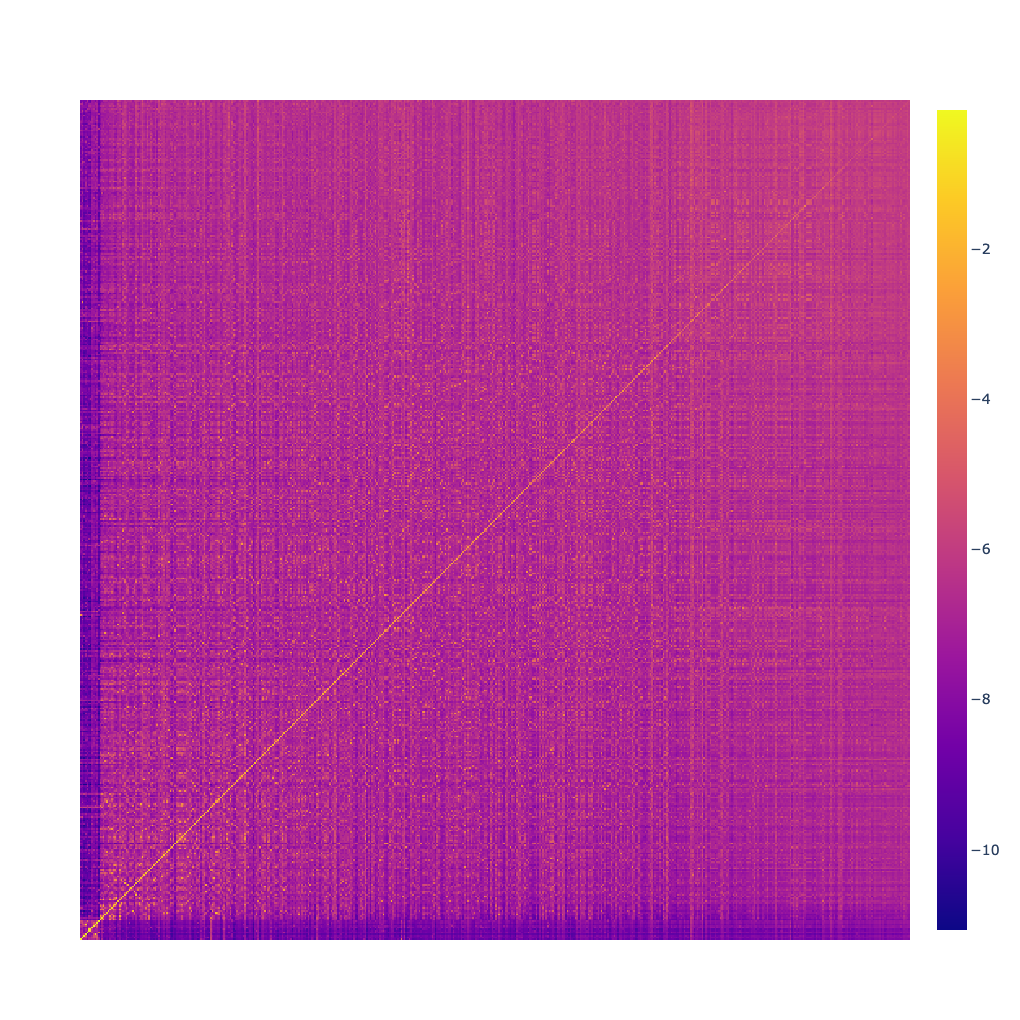
\includegraphics[width=\linewidth]{floats/confusion_lstm-3-1}
\caption{
  LMCC confusion matrix for the LSTM model with $l_c=1$, showing $\log(P(c_j\mid c_i))$, 
  with $c_i$ on the x-axis and $c_j$ on the y-axis.
  Communities are sorted by indiscernability.
  (The first few communities predominantly use a language other than English, and are thus very discernable.)}
\label{fig:confusion}
\end{figure}


But we want a more quantitative measure, corresponding to the ability of the LMCC to correctly
recognize messages coming from a given community $c_j$. We could use
something like an F-score, but we prefer to use a perplexity-like metric,
which is has stronger information-theoretic grounds.
To this end, we define the \emph{linguistic indiscernibility} of community $c_j$, 
noted $\Ind_j$. 
First, note that each row of $C$ is a probability distribution,
since it is computed as the average of $P(c=c_i \mid m)$ for $m\in M_j$.
The exponential of the entropy of the $j$th row of \(C\) is therefore a perplexity score,
whose maximum is the total number of communities (46 for us).
Thus we define $\Ind_j$ by scaling this perplexity by the number of communities:
\[\Ind_j = \frac{e^{-\sum_i C_{ij} log(C_{ij})}}{|C_j|}\]
This way $Ind_j=0$ means that the LMCC is completely certain of its
choice, while $Ind_j=1$ means that equal probability is given to all
predictions.  In general $\Ind_j$ is a score of uncertainty of the
LMCC, given messages from a community $c_j$.

Indiscernibility of a given community is a robust measure: it is
almost perfectly correlated across CCLMs (such as transformers, LSTM
and various values of $l_c$).  In fact, we observe a correlation
between the indiscernibility measures by every pair of models with
Pearson's $r \geq 0.96$ and $Bp < 0.0001$. 

However, we observe that community-wise perplexity is only weakly (if at all) 
correlated with community indiscernibility under the corresponding latent 
LMCC (see \cref{tab:ind-corrs} and, for example, \cref{fig:cclm-lmcc-ppl}).
In other words, the linguistic complexity of a given community
is a poor predictor of how distinctive its language is.
%
\begin{table}
  \small
  \centering
  \begin{tabular}{llrrrr}
  \toprule
      & $l_c$ & $\Ppl_{M_j}$ & $\IG_{M_j}$ \\
  \midrule
  \multirow{4}{*}{LSTM}         & 0 &            - &             - \\
                                & 1 &         0.19 &         -0.40 \\
                                & 2 &         0.19 &         -0.43 \\
                                & 3 &         0.06 &         -0.45 \\
  \midrule
  \multirow{4}{*}{Transformer}  & 0 &         0.19 &         -0.41 \\
                                & 1 &         0.23 &         -0.43 \\
                                & 2 &         0.16 &         -0.39 \\
                                & 3 &         0.12 &         -0.40 \\
  \bottomrule
  \end{tabular}
  \caption{ (TODO: missing data) Pearson's $r$ correlation coefficient between community
    indiscernibility ($\Ind_j$) and two different predictors: CCLM
    perplexity on messages from community $c_j$ ($\Ppl_{M_j}$), and
    CCLM information gain on messages from $c_j$ ($\IG_{M_j}$). $p < 0.001$
    for all correlations except $\Ppl_{M_j}$ for the LSTM with 
  $l_c=3$ ($p=0.218$) and Transfomer with $l_c=3$ ($p=0.010$).}
  \label{tab:ind-corrs}
\end{table}

\begin{figure*}
  \begin{tikzpicture}
  \begin{groupplot}[
    group style={group size=2 by 1},
    legend style={anchor=north, legend columns=1, font=\tiny},
    every node near coord/.append style={font=\sffamily\tiny},%
    axis x line*=bottom, axis y line*=left,
  ]
  \nextgroupplot[xlabel=$\Ppl_{M_j}$, ylabel=$\Ind_j$]
      \addplot+[%
        only marks,
        mark=*,
        mark options={scale=0.35, solid, color=violet!80, fill=violet},
        font=\tiny,
      ] table [x={lstm-3-1_ppl}, y={lstm-3-1_indisc}] {floats/comm.csv};
  \nextgroupplot[xlabel=$\IG_{M_j}$, ylabel=$\Ind_j$, xmax=1.6]
      \addplot+[%
        only marks,
        mark=*,
        mark options={scale=0.35, solid, color=violet!80, fill=violet},
        font=\tiny,
      ] table [x={lstm-3-1_ig}, y={lstm-3-1_indisc}] {floats/comm.csv};
  \end{groupplot}
  \end{tikzpicture}
  \caption{%
    Community indiscernibility (y-axis), 
    in relationship to linguistic complexity (left) and 
    CCLM information gain (right). Shown here for the LSTM
    model with $l_c=1$. See \cref{tab:ind-corrs} for 
    Pearson's r correlations for all models.
    (Communities with \(\IG > 1.6\) (3 outliers) are hidden to make the correlation easier to observe.)
  }
  \label{fig:cclm-lmcc-ppl}
\end{figure*}


% We could also check if communities are well-separated in the SNAP community encodings

On the other hand, community indiscernibility is correlated with
the information gain of the CCLM
on messages from that community's test set
(see \cref{tab:ind-corrs} and, for example, \cref{fig:cclm-lmcc-ppl}).
Communities for which the language model benefits most from 
the conditioned model are generally easier for the LMCC to classify.

Finally, we note that, even though community-conditioning affects
perplexity very little overall, it provides large benefits in term of
the underlying Bayesian classifier. Indiscernibility is on average
TODO with a standard deviation of TODO. Roughly speaking, this means
that, while the linguistic variations does not allow our model to
pinpoint the originating community of a message, it can often
eliminate TODO (a percentatge?) of communities as possible locations
for it. Further more, the information gain provided by
community-conditioning is a good predictor of how specific the
community is.



% Finally, we investigate the correlation between the stability of a
% community and the perplexity of the LMCC for it. Stability is defined as TODO.

% - compute pearson correlation coefficient

% We see a positive correlation: this suggests that the more stable a
% community is, the more difficult it is to identify message as coming
% from it. What this suggests is that stable communities tend to use a
% varied and standard, subset of English, while unstable communities
% resort to more formulaic language. This may suggests that to 'fit' in an
% unstable community, one must use more obvious linguistic cues than in
% a stable community. In fact, it is reasonable to think that a new
% member will ostensibly use community-specifc language, but once
% established in a community, a member would tend not to do so.


\jp{Conclusion: perplexity (linguistic complexity) is not correlated
  to how recognisable a community is. Presumably (in general) some very specific
  lexical items are characteristic of a community.}





\section{Social Analysis of CCLM community embeddings (TODO: better title)}

In this section we investigate whether (and how much) the community
embeddings obtained from the CCLMs correlate with the community-member
relationship on Reddit.

To this end, we compare the CCLM-learned community
embedding with the community embedding created by \citet{Kumar2018},
who generated them using using a negative-sampling optimization
algorithm and the message-community co-occurrence matrix as ground
truth, using data which spans January 2014 to April 2017.
We refer the reader
to \citet{Kumar2018}
for details, but the important point is that no linguistic
information is used to create these embeddings: they only reflect the social
relationship between communities, via 
the user-community membership relation. In contrast, CCLM community embeddings depend in no
way on which user is the author of any given message: we only use the
contents of messages, not authorship data.
%

\subsection{Comparing embeddings: method}
% Explain the problem (idea: comparing cosine similarities --> too much data, again)

Let us call \(L\) the matrix of (normed) linguistic embeddings and \(S\) the matrix
of (normed) social embeddings. Thus \(L_i\) and \(S_i\) are the linguistic and
social embeddings for community \(i\).

To compare embeddings, one might naively think that it suffices to
calculate the distance between two embeddings index-wise, which is
equal to the Frobenius distance between \(L\) and \(S\):

\[||L-S||_F = \sum_i (L_i - S_i)\]

The problem with this approach is that the dimensions of \(L\) and \(S\) may
not coincide. Applying a simple permutation of dimensions may widely
change the correlation metric. To make the metric resilient to such
effects, we can compute the minimum distance between \(L_i\) and \(S_i\), for
any orthogonal matrix \(\Omega\) applied to \(L\):

\[d(L,S) = \mathsf{argmin}_\Omega ||ΩL-S||_F\]

Computing \(d(L,S)\) is known as the orthogonal Procrustes problem~\citep{Gower2004}. The
solution is
\[d(L,S) = n - \mathsf {Tr} (Σ)\] where the matrix \(Σ\) is obtained by the singular value
decomposition \(U^TΣV = LS^T\). Additionally the vectors of \(U\) and \(V\) give
the directions of correlation respectively of \(L\) and \(S\). That is, each
singular value \(\sigma_i\) (the elements of the diagonal matrix \(Σ\)), give a measure of how much
correlation there is between the directions \(U_i\) and \(V_i\).

Further, we can apply a permutation to \(U\), \(V\) and \(Σ\) such
that \(σ_i > σ_j\) iff \(i < j\). Doing so, the largest singular value
\(σ_0\) corresponds to the principal directions of correlation
(\(U_0\), \(V_0\)), \(σ_1\) to the second principal direction, etc.

The \(d(L,S)\) metric ranges from \(0\) 
(corresponding to perfect correlation, 
obtained for example if \(L=S\)) 
to \(n\) 
(corresponding to perfect independence), 
where $n=510$ is the number of communities considered.

To get a more precise sense of what value of \(d(L,S)\) indicates significant correlation,
We have experimentally computed \(d(L,S)\) for five random  ``embeddings'' 
with the same shape as the CCLM embeddings.
We observed a mean of \(μ_d=431.39\) and a (Bessel's-corrected) 
standard deviation \(s_d=2.90\) in their distance from the social embedding, \(S\). %\jp{Unfortunate overloading} luckily it seems that sample stdev is often written with an $s$ to differentiate from population stdev


Thus if \(d(L,S)\) is below the mean by several standard deviations, we can safely
assume that there is statistically significant correlation between
\(L\) and \(S\).  This is the case: we observe a difference between 61 and 68 standard deviations
(\cref{tab:embedding-correlations}). Further, it is clear that the CCLM embedding
capture some of the same information as the social-network embeddings.
We also give a sense of \emph{how} the correlation is manifested by
analysis of the two principal components of correlation in the
linguistic embeddings, \(U_0\) and \(U_1\). To do so we plot the
projection of embeddings on along \(U_0\) and \(U_1\), together with
the corresponding singular values.\jp{TODO}

\begin{table}
\centering
\begin{tabular}{llcc}
\toprule
                        &   & LSTM     & Transformer \\
\midrule
  \multirow{4}{*}{$l_c$}  & 0 &         254.06  (61.21) &         239.41  (66.79)  \\
                          & 1 &         245.14  (64.29) & \textbf{232.18} (68.54)   \\
                          & 2 &         249.17  (62.90) &         233.47  (68.32)  \\
                          & 3 & \textbf{241.13} (65.67) &         237.74   (66.84) \\
\bottomrule
\end{tabular}
\caption{Distance between CCLM embeddings and the social network-based embedding
of \citet{Kumar2018}, as measured by $d(L,S)$. In parentheses is the number of standard deviations
from the mean distance of our random embedding samples.} \label{tab:embedding-correlations}
\end{table}

% (Another idea may be to correlate the cosine similarity between
% \((S_i,S_j)\) and \((L_i,L_j)\). But this would yield one number for
% each pair of communities \((510 × 509 / 2)\): too much data to deal with,
% and it is hard to get a sense of the meaning, let alone statistical significance of the
% resulting correlation coefficient.)\jp{Not sure if this discussion has its place here.}


\subsection{Results}

%    Results:
%      - Correlation between Kumar2018 and best LSTM
%      - Correlation between Kumar2018 and best Transformer 
%      - Correlation between Transformer and LSTM
%      - Concatenations ???


%\begin{figure*}[t]
%\begin{tikzpicture}
  %\begin{groupplot}[
    %group style={group size=2 by 1},
    %yticklabels={,,}, xticklabels={,,},
    %legend style={anchor=north, legend columns=1, font=\sffamily\tiny},
  %]
    %\nextgroupplot
    %\commscatter{lstm-3-1_pca1}{lstm-3-1_pca2}
    %\nextgroupplot
    %\commscatter{transformer-3-3_pca1}{transformer-3-3_pca2}
    %\legend{General interest,Videogames,Technology,Sports,Female-focused,Other}
  %\end{groupplot}
%\end{tikzpicture}
%\caption{Plot of embeddings along the 2 principal dimensions of correlation between .... TODO of an LSTM (left, $c=1$) and transformer (right, $c=3$) model.
%Color correspond the 5-means clustering of .... TODO}
%\label{fig:comm-pca}
%\end{figure*}




\section{Related work}

We have presented results using conditional neural language models
to model variation between speech communities.
The architecture of these models concatenates a vector representation
of the conditioned variable to the input of the sequence model.
This approach has been applied in various conditioned text generation domains such as 
image captioning \citep{Vinyals2015}, machine translation \citep{Kalchbrenner2013},
but it has not, to our knowledge, been used extensively to study linguistic variation.

There are, however, related applications of conditional neural language models.
\citet{Lau2017a} presents a neural language model that jointly learns to predict
words on the sentence-level and represent topics on the document level.
The topic representation is then fed back into the language model, 
improving its performance on next word prediction.
This is similar to how our model experiences improved performance
by learning community representations. 
Unlike our model, topics are inferred in an unsupervised way, 
raising the question of whether communities could be identified from 
unlabeled data as well.

Along these lines, \citet{OConnor2010} uses a Bayesian generative
model to infer communities from variation in text data.  In contrast
to our work, this model treats words as independent events, ignoring
the structure (and variation) in the construction of sequences.  It
does further suggest, however, that community-level variation can be
modeled in an unsupervised way.

\section{Discussion and Conclusion}


% \jp{I propose that most of the following analysis should be spread between the relevant sections, and only have a tiny summary here + future work.}
To sum up our findings, 
we observed that various communities exhibit widely varying levels of
linguistic complexity \ref{hyp:varying-complexity}, with perplexity
per-word ranging from less than 34 to more than 65 for the best model 
architecture.

With indiscernibility values evenly ranging over the whole possible
range (1 to 510), we find that CCLMs can be used to recognize certain
communities based on latent Bayesian classification
\ref{hyp:LMCC-works}, but not all.  We cannot rule out that generic
communities exhibit distinctive linguistic patterns, but none of our
CCLMs are able to discern them. In contrast, the distinctive patterns
of narrow-topic communities are just as recognizable by all our LSTM
and Transformer models.

We find a mild correlation (\cref{tab:ind-corrs}) between the
perplexity of the CCLM and the indiscernibility of the corresponding
community \ref{hyp:rich-harder-to-identify}, with factors ranging from
0.06 to 0.23. However, The trend is more clear when considering the
correlation with information gain and indiscernibility (correlation
from 0.39 to 0.46). So this means that, when trying to identify a
community, it is not its absolute perplexity that matters, but rather
the difference in perplexity with the baseline.

We find that the layer at which the community embedding is taken into
account in a CCLM influences its perplexity \ref{hyp:layer-effect},\jp{Delete this hypothesis?}
albeit weakly. For LSTM models, the perplexity per word, averaged over
messages from all communities, varies between \num{49.60} and \num{50.83}. (with \num{51.99} for the\jp{update numbers?}
unconditioned model) The perplexity per word is slightly higher for
$l_c=0$, and has very little difference between the other models, with
$l_c=3$ being the best.  For transformer models, it varies between 
\num{52.28} and \num{78.76}. Here perplexity per-word is clearly not a monotonous
function of $l_c$: the maximum is reached at $l_c=2$. We did not
expect non-monotonicity, and leave studying this effect to future
work.

The pattern of information gain by community is similar across
architectures.  Communities that benefit most from the conditioned
model behave that way for both the LSTM and transformer.  However,
there are some differences.  For example, the subreddit
\emph{relationships} has an information gain of \num{1.018} for the
best CCLM LSTM but only \num{0.998} for the best transformer model.
Why was the LSTM able to take advantage of the community information
for this community, where the transformer was not?  It would be
interesting to investigate these differences in future work, since it
could reveal differences in the kind of linguistic variation the
different model architectures capture.\jp{update?}

The representation of communities built by CCLM exhibits a clear
correlation with user co-occurrence patterns
\ref{hyp:extra-linguistic-correlation}. A natural
question that may arise is how much this correlation can be explained by
user-specific linguistic patterns. We plan to control for this variable
in future work, for example by building author-conditioned language
models and testing if community vector embeddings can be determined by
the set of the vector embeddings of its members.

\bibliography{paper}
\bibliographystyle{acl_natbib}

\end{document}

% LocalWords:  CCLMs Gumperz NLP Hovy Ciot Bamman DelTredici CFB SMU
% LocalWords:  cancelled pre emptively CCLM Reddit subreddits dataset
% LocalWords:  preprocessed tokenized SpaCy tokenizer Honnibal LSTM
% LocalWords:  Hochreiter Vaswani softmax un AdamW Loshchilov IG Ppl
% LocalWords:  LM videogame embeddings PCA Kumar lstm LMCC ij th Lau
% LocalWords:  indiscernibility Vinyals Kalchbrenner OConnor
% LocalWords:  monotonicity subreddit Frobenius
